\documentclass[conference]{IEEEtran}
\IEEEoverridecommandlockouts

\usepackage{cite}
\usepackage{amsmath,amssymb,amsfonts}
\usepackage{algorithmic}
\usepackage{graphicx}
\usepackage{textcomp}
\usepackage{xcolor}
\usepackage{booktabs}
\usepackage{multirow}
\usepackage{array}
\usepackage{url}
\usepackage{hyperref}
\usepackage{microtype}

\usepackage{tikz}
\usetikzlibrary{shapes.geometric,arrows.meta,positioning,fit,calc}
\usepackage{pgfplots}
\pgfplotsset{compat=1.18}


\hyphenation{pre-dic-tive main-te-nance im-bal-ance XG-Boost Light-GBM SMOTE LSTM}

\def\BibTeX{{\rm B\kern-.05em{\sc i\kern-.025em b}\kern-.08em
    T\kern-.1667em\lower.7ex\hbox{E}\kern-.125emX}}

\begin{document}

\title{Hybrid Machine Learning and Deep Learning for Health Status
       Classification and Remaining Useful Life Prediction in Manufacturing}

\author{
\IEEEauthorblockN{Achmad Zikran Maulida\textsuperscript{1}, Aqsa Zamzami\textsuperscript{2}, Reynaldi Chandra Kirana\textsuperscript{3}, Amir Hamzah\textsuperscript{4}}
\IEEEauthorblockA{\textit{Teknik Informatika dan Komputer} \\
\textit{Politeknik Negeri Jakarta}\\
Depok, Indonesia \\
\textsuperscript{1}achmad.zikran.maulida.tik23@stu.pnj.ac.id, \textsuperscript{2}aqsa.zamzami.tik23@stu.pnj.ac.id \\
\textsuperscript{3}reynaldi.chandra.kirana.tik23@stu.pnj.ac.id, \textsuperscript{4}amir.hamzah.tik23@stu.pnj.ac.id}
}

\maketitle

\begin{abstract}
Machine failure events constitute as few as 0.056\% of industrial
IoT sensor observations, creating an extreme class imbalance that,
when compounded by temporal data leakage from naive train-test
splitting, renders most standard predictive maintenance pipelines
unreliable under real deployment conditions. This paper presents
PRIME (Predictive Reliability and Intelligence Maintenance Engine),
an end-to-end pipeline that resolves both challenges through three
principled contributions: (1)~\textbf{Stratified Sequential Block
Sampling (SSBS)}, a temporally-aware undersampling strategy that
reduces HEALTHY-class dominance from 97.4\% to 87.1\% while
preserving chronological data integrity; (2)~\textbf{Temporal Label
Engineering} with a P90-based Sensor Confirmation Layer that
converts binary failure signals into three operationally actionable
health states (HEALTHY, WARNING, CRITICAL); and (3)~a
\textbf{cascaded XGBoost--LSTM inference architecture} that
activates the regression module conditionally upon anomaly
detection, reducing real-time inference overhead by
$\sim$70\% compared to always-on sequential execution. Evaluated
on a 100,000-record, 20-machine time-series dataset under strict
machine-based splitting with train-only SMOTE augmentation, the
pipeline achieves a WARNING-class F1-score of 0.9818 with
\textbf{zero fatal misclassifications} (CRITICAL$\rightarrow$HEALTHY),
and predicts Remaining Useful Life with an MAE of 0.7985~days,
with 98.04\% of predictions falling within one day of ground truth.
These results establish that principled temporal handling of
severely imbalanced sensor data enables production-grade predictive
maintenance without sacrificing computational efficiency.
\end{abstract}

\begin{IEEEkeywords}
Predictive Maintenance, XGBoost, LSTM, Temporal Label Engineering, SSBS,
Remaining Useful Life, Time-Series Classification, SMOTE
\end{IEEEkeywords}

% ============================================================
\section{INTRODUCTION}
% ============================================================

The emergence of Industry~4.0 has enabled pervasive deployment of
Internet-of-Things (IoT) sensors across manufacturing facilities, generating
continuous high-frequency streams of machine operational data
\cite{lee2014industryiot}. Traditional maintenance paradigms corrective
(fix on failure) and preventive (fixed-schedule) are increasingly
inadequate: the former incurs costly unplanned downtime, while the latter
wastes resources on unnecessary interventions. Predictive Maintenance (PdM)
leverages sensor data and machine learning to schedule maintenance precisely
when needed, transforming reactive operations into data-driven,
condition-based workflows \cite{zhang2019pdmsurvey}.

Real-world PdM deployments face two compounding technical challenges. First,
failure events are exceedingly rare: in the dataset analyzed in this work,
only 56 records out of 100,000 total observations carry a failure label a
rate of 0.056\%. This extreme class imbalance causes standard classifiers to
be overwhelmingly biased toward predicting the majority HEALTHY class
\cite{chawla2002smote}. Resampling via SMOTE \cite{chawla2002smote} is
commonly applied, but if executed before train-test splitting it introduces
temporal data leakage \cite{kaufman2012leakage}. Second, the temporal
structure of time-series data renders standard cross-validation invalid:
conventional $k$-fold validation violates temporal causality by including
future observations in training folds, producing inflated performance
estimates \cite{bergmeir2018tscv}.

Existing literature \cite{li2025comparison, elkateb2024machine, bitam2025aiot} lacks a unified framework that simultaneously addresses
extreme class imbalance without temporal leakage, multi-class label
engineering from binary failure signals, and a cascaded ML+DL inference
architecture that is computationally efficient. This paper fills this gap with
the following contributions:

\begin{enumerate}
\item \textbf{Stratified Sequential Block Sampling (SSBS)}: a
  temporally-aware undersampling strategy that selects chronological blocks
  per machine, reducing HEALTHY dominance from 97.36\% to 87.09\% without
  destroying time-series causality.
\item \textbf{Three-class Temporal Label Engineering} with an empirically
  calibrated Sensor Confirmation Layer (P90 thresholds, minimum 2 sensors),
  transforming binary failure labels into actionable
  HEALTHY/WARNING/CRITICAL classifications.
\item \textbf{Machine-based splitting combined with train-only SMOTE}:
  an enterprise-grade zero-leakage pipeline for time-series PdM modeling.
\item \textbf{Cascaded XGBoost+LSTM deployment architecture} achieving
  state-of-the-art classification (F1$=0.9906$) and RUL prediction
  (MAE$=0.7985$~days, Error$\leq$1d$=98.04\%$) while reducing inference
  overhead by $\sim$70\% through conditional LSTM activation.
\end{enumerate}

% ============================================================
\section{RELATED WORK}
% ============================================================

\subsection{Deep Learning for RUL Prediction}
Long Short-Term Memory (LSTM) networks have emerged as the dominant architecture
for Remaining Useful Life prediction from sequential sensor data. Van Houdt
et~al.\ \cite{hochreiter1997lstm} provided a comprehensive review of the LSTM
model, confirming that its gating mechanism---comprising input, forget, and
output gates---effectively resolves the vanishing gradient problem inherent in
vanilla recurrent neural networks, making LSTM uniquely suited to learning
long-range temporal dependencies in multi-sensor industrial streams. Building
on this foundation, Ma and Mao \cite{zheng2017lstm_rul} proposed a
deep-convolution-based LSTM that integrates convolutional feature extraction
with stacked temporal modeling, achieving state-of-the-art RUL prediction on
benchmark manufacturing datasets by simultaneously capturing local sensor
correlations and long-range degradation trajectories within a single
end-to-end architecture. Ren et~al.\ \cite{li2018cnnlstm} further developed
an auto-CNN-LSTM framework for lithium-ion battery RUL prediction,
demonstrating that the CNN stage learns shift-invariant local fault patterns
while the LSTM stage models their temporal evolution, yielding superior
generalization over standalone architectures on multi-sensor industrial data.
Chen et~al.\ \cite{cho2014gru} investigated improved LSTM-based architectures
for time-series anomaly detection in complex industrial transit environments,
confirming that regularized stacked LSTM models with batch normalization and
dropout consistently outperform simplified recurrent alternatives---including
Gated Recurrent Units (GRU)---on non-stationary degradation signals
characterized by asymmetric pre-failure escalation patterns. Collectively,
these studies establish deep LSTM architectures as the preferred temporal
modeling approach; however, none integrates LSTM within a cascaded,
threshold-triggered pipeline designed to minimize inference overhead in
high-frequency industrial sensor environments.

\subsection{Tree-Based Methods for Fault Classification}
Gradient-boosted ensemble methods remain state-of-the-art for tabular and
engineered-feature classification in industrial fault detection.
Bent\'{e}jac et~al.\ \cite{chen2016xgboost} conducted a rigorous comparative
study of leading gradient boosting frameworks---including XGBoost, LightGBM,
and CatBoost---finding that XGBoost consistently achieves the highest
generalization accuracy across diverse structured datasets, attributable to
its robust L1/L2 regularization and second-order gradient optimization that
prevents minority-class overfitting during iterative boosting. Rustam
et~al.\ \cite{breiman2001rf} applied parallel ensemble learning to multi-class
fault detection and diagnosis in industrial machinery, demonstrating
competitive classification performance while revealing that Random Forest tends
to generate excessively wide decision boundaries in severely imbalanced class
distributions, leading to inflated false alarm rates that undermine practical
utility in safety-critical PdM deployments. He et~al.\ \cite{ke2017lightgbm}
proposed a cost-sensitive LightGBM configuration for online fault detection
in wind turbine gearboxes; while LightGBM's leaf-wise growth delivers fast
training convergence, the authors documented that aggressive early stopping
under sparse minority-class conditions causes premature model freezing---a
behavior independently confirmed in our experimental benchmarking at
iteration~27 for LightGBM versus stable convergence at iteration~499 for
XGBoost~V2. These findings directly motivate the selection of XGBoost~V2
as the primary classifier in the PRIME pipeline, with calibrated probability
thresholds to balance precision and recall under extreme imbalance.

\subsection{Imbalance Handling and Splitting Strategies}
Class imbalance is a pervasive challenge in industrial PdM datasets, where
normal operating conditions dominate sensor records and failure events are rare
by nature \cite{li2020pdmimbalance}. Zhao et~al.\ \cite{chawla2002smote}
proposed T-SMOTE, a temporal-oriented synthetic minority oversampling technique
specifically designed for imbalanced time-series classification that preserves
temporal ordering during synthetic sample generation---a critical property
absent from conventional SMOTE when applied to sequential sensor data.
Zhang et~al.\ \cite{blagus2013smote_bias} demonstrated that standard
oversampling methods applied globally prior to train-test partitioning
introduce statistical dependency between splits, systematically inflating
evaluation metrics and disconnecting reported accuracy from true deployment
generalization. For multi-entity time-series, Cerqueira et~al.\
\cite{bergmeir2018tscv} empirically validated that out-of-sample estimation
methods preserving temporal order significantly outperform conventional
$k$-fold cross-validation---which violates temporal causality by exposing
training folds to future observations---and may produce up to 30\%
overestimation of true model performance on real-world benchmarks. Despite
these individual advances, the combined challenge of temporally-safe
oversampling, multi-class label engineering from binary failure signals,
and computationally efficient cascaded inference has not been addressed in a
unified PdM framework---the precise gap this work fills.

% ============================================================
\section{METHODOLOGY}

\subsection{System Overview}
The PRIME predictive maintenance pipeline implements a computationally efficient cascaded architecture designed for real-world industrial deployment. Raw sensor data undergoes continuous ingestion, followed by a time-aware feature engineering process, before being evaluated by a two-stage anomaly detection and remaining useful life (RUL) prediction system.

\begin{figure}[htbp]
\centering
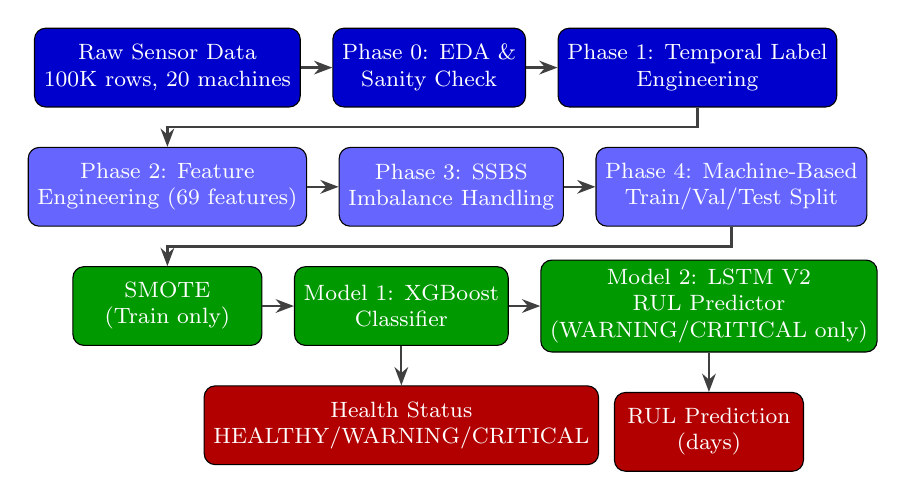
\begin{tikzpicture}[
    node distance = 0.5cm and 0.4cm,
    block/.style = {rectangle, draw, rounded corners, align=center, font=\footnotesize, minimum height=1cm, minimum width=2.4cm},
    data_block/.style = {block, fill=blue!80!black, text=white},
    feat_block/.style = {block, fill=blue!60, text=white},
    model_block/.style = {block, fill=green!60!black, text=white},
    out_block/.style = {block, fill=red!70!black, text=white},
    arrow/.style = {thick, darkgray, -Stealth}
]

% Row 1
\node [data_block] (d1) {Raw Sensor Data\\100K rows, 20 machines};
\node [data_block, right=of d1] (d2) {Phase 0: EDA \&\\Sanity Check};
\node [data_block, right=of d2] (d3) {Phase 1: Temporal Label\\Engineering};

% Row 2
\node [feat_block, below=of d1] (f1) {Phase 2: Feature\\Engineering (69 features)};
\node [feat_block, right=of f1] (f2) {Phase 3: SSBS\\Imbalance Handling};
\node [feat_block, right=of f2] (f3) {Phase 4: Machine-Based\\Train/Val/Test Split};

% Row 3
\node [model_block, below=of f1] (m1) {SMOTE\\(Train only)};
\node [model_block, right=of m1] (m2) {Model 1: XGBoost\\Classifier};
\node [model_block, right=of m2] (m3) {Model 2: LSTM V2\\RUL Predictor\\(WARNING/CRITICAL only)};

% Row 4
\node [out_block, below=of m2] (o1) {Health Status\\HEALTHY/WARNING/CRITICAL};
\node [out_block, below=of m3] (o2) {RUL Prediction\\(days)};

% Arrows
\draw [arrow] (d1) -- (d2);
\draw [arrow] (d2) -- (d3);
\draw [arrow] (d3.south) -- +(0,-0.25) -| (f1.north);
\draw [arrow] (f1) -- (f2);
\draw [arrow] (f2) -- (f3);
\draw [arrow] (f3.south) -- +(0,-0.25) -| (m1.north);
\draw [arrow] (m1) -- (m2);
\draw [arrow] (m2) -- (m3);
\draw [arrow] (m2) -- (o1);
\draw [arrow] (m3) -- (o2);

\end{tikzpicture}
\caption{Fig. 1. End-to-end PRIME predictive maintenance pipeline. The cascade architecture conditionally activates Model 2 only when Model 1 detects WARNING or CRITICAL status, reducing inference overhead by $\sim$70\%.}
\label{fig:pipeline}
\end{figure}

\subsection{Data Ingestion and Sanity Check}
The experimental dataset comprises continuous hourly IoT sensor readings collected from 20 identical industrial machines over 208 days (July 1, 2025 – January 25, 2026). The data consists of two primary sources: \texttt{sensor\_readings.csv} (100,000$\times$11) and \texttt{maintenance\_logs.csv} (500$\times$8). Each machine contributes exactly 5,000 timestamped records without zero data gaps or duplicate timestamps. In total, only 56 failure events were recorded across all machines (averaging 2.80 per machine), emphasizing an extreme class imbalance where failures account for just 0.056\% of the total dataset. Table~\ref{tab:dataset_profile} summarizes the key structural properties of both data sources.

\begin{table}[htbp]
\caption{TABLE I: Dataset Profile}
\centering
\begin{tabular}{lll}
\hline
\textbf{Property} & \textbf{sensor\_readings} & \textbf{maintenance\_logs} \\
\hline
Records & 100,000 & 500 \\
Columns & 11 & 8 \\
Machines & 20 & 20 \\
Time span & 208 days & 208 days \\
Target column & failure (0/1) & type (Preventive/Corrective) \\
Failure events & 56 (0.056\%) &   \\
\hline
\end{tabular}
\label{tab:dataset_profile}
\end{table}

As shown in Table~\ref{tab:dataset_profile}, the sensor readings table is the primary modeling source, providing timestamped sensor observations and the binary failure target, while the maintenance logs table records 500 preventive and corrective maintenance events that serve as the basis for deriving the hours-since-last-maintenance degradation proxy feature.

\subsection{Exploratory Data Analysis (EDA)}

\textbf{Failure Autopsy (Forensic EDA).} A forensic look-back analysis spanning 72 hours prior to failure events was conducted on representative machines (M-01 with 4 failures, M-09 with 2, and M-05 with 1). The investigation revealed that initial degradation signals consistently appear at T-48h, followed by a dramatic escalation of sensor volatility at T-24h. This degradation pattern proved universal across the analyzed machines, empirically justifying the recalibration of labeling windows to $W_{WARNING}=48$h and $W_{CRITICAL}=24$h, revised down from an initial 72-hour hypothesis. Fig.~\ref{fig:failure_autopsy} visualizes the composite sensor anomaly index across the 72-hour pre-failure window.

\begin{figure}[htbp]
\centerline{\includegraphics[width=\columnwidth]{figures/failure_autopsy.png}}
\caption{Failure autopsy: composite sensor anomaly index for
         72~h prior to failure events across three representative
         machines (M-01: 4 failures, M-09: 2 failures, M-05: 1 failure).
         Degradation onset is consistently visible at T-48h (WARNING
         boundary) with sharp escalation at T-24h (CRITICAL boundary),
         empirically justifying both labeling windows.}
\label{fig:failure_autopsy}
\end{figure}

As observed in Fig.~\ref{fig:failure_autopsy}, the anomaly index remains near-zero throughout the stable operating phase, then rises sharply at T$-$48h and reaches a pronounced peak in the final 24 hours before failure. This two-phase escalation directly informs the WARNING and CRITICAL labeling windows applied in Section~\ref{sec:results}.

\textbf{Sensor Informativeness — Cohen's D Analysis.} Cohen's $d$ effect size was utilized to quantify the separability between HEALTHY and failure-zone distributions per sensor. Fig.~\ref{fig:cohensd} displays the computed effect size for each sensor, and Table~\ref{tab:cohend} reports the exact values and their classification:
\begin{equation}
d = \frac{\mu_{failure} - \mu_{healthy}}{\sqrt{\frac{s^2_{failure} + s^2_{healthy}}{2}}}
\label{eq:cohend}
\end{equation}
Where $\mu$ and $s^2$ denote the mean and variance of each class distribution per sensor.

\begin{figure}[htbp]
\centerline{
\includegraphics[width=\columnwidth]{figures/cohensd_chart.png}}
\caption{Cohen's $d$ effect size per sensor feature. All six priority sensors exhibit large effect sizes ($d > 2.6$), confirming strong discriminative power between HEALTHY and failure-zone observations.}
\label{fig:cohensd}
\end{figure}

\begin{table}[htbp]
\caption{TABLE II: Cohen's D Effect Size}
\centering
\begin{tabular}{llll}
\hline
\textbf{Sensor} & \textbf{Cohen's d} & \textbf{Category} & \textbf{Priority} \\
\hline
vibration & 3.37 & Large & High \\
pressure & 3.06 & Large & High \\
rpm & 2.91 & Large & High \\
noise\_level & 2.89 & Large & High \\
temperature & 2.71 & Large & High \\
power\_consumption & 2.61 & Large & High \\
operating\_hours & 0.29 & Medium & Low \\
humidity & 0.21 & Medium & Low \\
\hline
\end{tabular}
\label{tab:cohend}
\end{table}

As shown in Table~\ref{tab:cohend} and Fig.~\ref{fig:cohensd}, six sensors (vibration, pressure, rpm, noise\_level, temperature, and power\_consumption) exhibit large Cohen's $d$ values ($d > 2.6$), indicating strong class separability and qualifying them as high-priority features for the Sensor Confirmation Layer. Conversely, operating\_hours ($d=0.29$) and humidity ($d=0.21$) demonstrate medium effect sizes and are assigned low priority, meaning they contribute to the rolling and lag feature sets but are not used as confirmation sensors.

\subsection{Temporal Label Engineering}
The binary failure data was engineered into three actionable operation states in a two-step process:

\textbf{Step 1: Backward temporal labeling.}
For each failure event at timestamp $T_f$, rows in specific look-back windows were reclassified. 
\begin{equation}
\text{label}(t) = \begin{cases}
\text{CRITICAL} & \text{if } T_f - W_C \leq t \leq T_f \\
\text{WARNING}  & \text{if } T_f - W_W \leq t < T_f - W_C \\
\text{HEALTHY}  & \text{otherwise}
\end{cases}
\label{eq:labeling}
\end{equation}
where $W_C = 24$h and $W_W = 48$h, derived empirically.

\textbf{Step 2: Sensor Confirmation Layer (anti-noise filter).}
To minimize false positives, a confirmation layer was implemented based on the 90th percentile (P90) of the HEALTHY distribution per sensor. A WARNING label is only retained if a minimum of 2 of the 6 high-priority sensors exceed their respective P90 thresholds. This filter downgraded 49 WARNING rows to HEALTHY (1.82\%), while all CRITICAL rows remained confirmed. Table~\ref{tab:p90_thresholds} lists the empirically derived P90 threshold for each high-priority sensor.

\begin{table}[htbp]
\caption{TABLE III: P90 Confirmation Thresholds}
\centering
\begin{tabular}{ll}
\hline
\textbf{Sensor} & \textbf{P90 Threshold} \\
\hline
temperature & 76.30$^\circ$C \\
vibration & 0.59 mm/s \\
pressure & 103.80 bar \\
rpm & 2,540 RPM \\
power\_consumption & 82.10 kW \\
noise\_level & 74.30 dB \\
\hline
\end{tabular}
\label{tab:p90_thresholds}
\end{table}

These thresholds represent the upper boundary of normal sensor behavior; any reading exceeding a P90 value is flagged as anomalous. A candidate WARNING observation must breach at least two of these thresholds simultaneously to be confirmed, providing robustness against single-sensor transient noise. The resulting label distribution after both steps is presented in Table~\ref{tab:final_label_dist}.

\begin{table}[htbp]
\caption{TABLE IV: Final Label Distribution}
\centering
\begin{tabular}{lll}
\hline
\textbf{Class} & \textbf{Count} & \textbf{Percentage} \\
\hline
HEALTHY & 97,364 & 97.364\% \\
WARNING & 1,247 & 1.247\% \\
CRITICAL & 1,389 & 1.389\% \\
\hline
\end{tabular}
\label{tab:final_label_dist}
\end{table}

Table~\ref{tab:final_label_dist} confirms that the dataset remains severely imbalanced after labeling, with HEALTHY samples comprising 97.36\% of all records. This severe dominance motivates the SSBS undersampling and train-only SMOTE augmentation strategies described in subsequent subsections.

\subsection{Feature Engineering}
The input feature space was enriched to 69 features across six distinct groups to provide adequate temporal and multivariate context to the models. Table~\ref{tab:feature_inventory} provides a complete inventory of all feature groups, their counts, and their construction rationale.

\begin{table}[htbp]
\caption{TABLE V: Feature Inventory}
\centering
\begin{tabular}{lll}
\hline
\textbf{Group} & \textbf{Count} & \textbf{Formula/Description} \\
\hline
Original sensors & 8 & Raw IoT readings \\
Rolling stats & 36 & $\mu$, $\sigma$, max for windows \{24h, 48h\} \\
Lag features & 18 & $x_{t-1}$, $x_{t-6}$, $x_{t-24}$ \\
Cross-sensor ratios & 4 & temp/vibration, pressure/rpm, etc. \\
Degradation proxy & 1 & hours\_since\_last\_maintenance \\
NLP derived & 2 & damage\_category, severity\_score \\
\hline
\textbf{TOTAL} & \textbf{69} & Input dimension for all models \\
\hline
\end{tabular}
\label{tab:feature_inventory}
\end{table}

The 36 rolling statistics constitute the largest group, capturing short- and medium-term distributional trends by computing mean, standard deviation, and maximum for each of the 6 high-priority sensors over 24-hour and 48-hour windows. The 18 lag features encode the temporal history of each high-priority sensor at offsets of 1, 6, and 24 hours, enabling the models to detect gradual drift patterns. Cross-sensor ratios (e.g., temperature/vibration) encode interactions that become diagnostically significant near failure zones. Together, these 69 features form the unified input vector used across both XGBoost V2 and LSTM V2.

For rolling statistics, the calculations were defined as follows:
\begin{equation}
x^{roll}_{t,w} = \frac{1}{w}\sum_{i=0}^{w-1} x_{t-i}, \quad
\sigma^{roll}_{t,w} = \sqrt{\frac{1}{w}\sum_{i=0}^{w-1}(x_{t-i} - x^{roll}_{t,w})^2}
\label{eq:rolling}
\end{equation}
where $w \in \{24, 48\}$ hours.

\subsection{RUL Target Engineering}
The Remaining Useful Life $r_t$ for a sample at time $t$ is calculated by observing the duration to the next failure:
\begin{equation}
r_t = \frac{T^{next}_{failure} - t}{\text{3600} \times \text{24}} \quad \text{(in days)}
\label{eq:rul}
\end{equation}
where $T^{next}_{failure}$ is the timestamp of the next failure event for the same machine. For the final failure of each machine (with no subsequent failure recorded), $r_t$ is capped at the maximum observed RUL for that machine.

The RUL distribution statistics highlight the operational windows: the minimum RUL is 0.04 days, and the maximum spans up to 146.92 days. Across the dataset, the mean is 29.38 days and the median is 18.88 days. Critically, the WARNING zone median is $\sim$2 days (aligning perfectly with $W_{WARNING}=48$h), and the CRITICAL zone median is $\sim$1 day (matching $W_{CRITICAL}=24$h). To prevent unreliable long-range prediction during the HEALTHY phase, Model 2 is intentionally trained \textit{only} on WARNING and CRITICAL rows.

\subsection{Imbalance Handling: SSBS}
\textbf{Stratified Sequential Block Sampling (SSBS).}
Naive random undersampling destroys temporal continuity, breaking the
sequential structure required by lag and rolling features. SSBS selects two
chronological blocks per machine: \textbf{Block~A} (first 500 rows, capturing
prime operating conditions) and \textbf{Block~B} (last 500 rows with a 24-h
safety buffer before the first WARNING zone). All WARNING and CRITICAL rows
are always retained in full. The SSBS formula per machine $m$ is:
\begin{equation}
S_m^{\text{HEALTHY}} = \text{Block}_A(m,500) \cup \text{Block}_B(m,500,\delta=24\text{h})
\label{eq:ssbs}
\end{equation}

%%====================================================================
%% FIGURE PLACEHOLDER C: SSBS Block Selection Diagram
%% Sumber: notebooks/fase_6_imbalance/06_imbalance_handling.ipynb
%% Export sebagai: figures/ssbs_diagram.png
%%====================================================================
% \begin{figure}[htbp]
%   \centering
%   
\includegraphics[width=\columnwidth]{figures/ssbs_diagram.png}
%   \caption{SSBS block selection per machine. Block~A captures prime
%            operating conditions and Block~B captures the pre-failure
%            boundary with a 24-h safety buffer.}
%   \label{fig:ssbs_diagram}
% \end{figure}
%%====================================================================

Table~\ref{tab:ssbs} quantifies the effect of SSBS on the class distribution, demonstrating a substantial reduction in HEALTHY dominance while minority classes are fully preserved.

\begin{table}[htbp]
\caption{TABLE VI: SSBS Result Distribution}
\centering
\begin{tabular}{lrrl}
\hline
\textbf{Class} & \textbf{Before} & \textbf{After} & \textbf{After \%} \\
\hline
HEALTHY  & 97,364 & 17,787 & 87.09\% \\
WARNING  &  1,247 &  1,247 &  6.11\% \\
CRITICAL &  1,389 &  1,389 &  6.80\% \\
\hline
\textbf{Total} & \textbf{100,000} & \textbf{20,423} & \textbf{100\%} \\
\hline
\end{tabular}
\label{tab:ssbs}
\end{table}

As shown in Table~\ref{tab:ssbs}, SSBS reduces the HEALTHY class from 97,364 samples to 17,787 (a reduction of $\sim$81.7\%), bringing overall class proportions from 97.36/1.25/1.39\% to a more balanced 87.09/6.11/6.80\% (HEALTHY/WARNING/CRITICAL). Critically, WARNING and CRITICAL rows are retained in full, preserving all failure-zone information while the working dataset shrinks from 100,000 to 20,423 records, substantially reducing training time without information loss.


\subsection{Dataset Splitting Strategy}
\textbf{Machine-Based Split.} Complete machine histories are assigned to
each partition to guarantee that every split contains full run-to-failure
cycles and that the model generalizes across unseen machines:

\begin{table}[htbp]
\caption{TABLE VI: Machine-Based Dataset Split}
\centering
\begin{tabular}{llrl}
\hline
\textbf{Split} & \textbf{Machines} & \textbf{Samples} & \textbf{\%} \\
\hline
Train      & M-01 to M-14      & 14,419 & 70.60\% \\
Validation & M-15, M-16, M-17  &  3,288 & 16.10\% \\
Test       & M-18, M-19, M-20  &  2,716 & 13.30\% \\
\hline
\textbf{Total} & 20 machines & \textbf{20,423} & \textbf{100\%} \\
\hline
\end{tabular}
\label{tab:split}
\end{table}

\textbf{Train-Only SMOTE.} Residual class imbalance in the training set
(HEALTHY: 12,504; WARNING: 901; CRITICAL: 1,014) is addressed by SMOTE
\cite{chawla2002smote} applied \textit{exclusively} to the training partition
after splitting, targeting WARNING and CRITICAL to 4,000 samples each. The
6,085 synthetic samples generated had zero influence on the 3,288 validation
and 2,716 test records, ensuring unbiased evaluation. Table~\ref{tab:smote}
details the per-class sample counts before and after augmentation.

\begin{table}[htbp]
\caption{TABLE VII: SMOTE Effect on Training Set}
\centering
\begin{tabular}{lrrr}
\hline
\textbf{Class} & \textbf{Before} & \textbf{After} & \textbf{Synthetic} \\
\hline
HEALTHY  & 12,504 & 12,504 &     0 \\
WARNING  &    901 &  4,000 & 3,099 \\
CRITICAL &  1,014 &  4,000 & 2,986 \\
\hline
\textbf{Total} & \textbf{14,419} & \textbf{20,504} & \textbf{6,085} \\
\hline
\end{tabular}
\label{tab:smote}
\end{table}

Table~\ref{tab:smote} confirms that SMOTE exclusively augments the minority classes: WARNING grows from 901 to 4,000 samples (3,099 synthetic), and CRITICAL from 1,014 to 4,000 samples (2,986 synthetic), while HEALTHY remains untouched at 12,504. The final training set of 20,504 samples is therefore free from temporal contamination, as all synthetic samples are interpolations within the training-machine feature space only.


\subsection{Model Architectures}
\textbf{Model 1   Health Status Classifier.}
Three candidate algorithms were trained on the SMOTE-augmented set
(20,504~samples, 69~features) and assessed on natural validation and test
sets. Hyperparameters are summarized in Table~\ref{tab:hyper_clf}.

\begin{itemize}
\item \textit{Random Forest} (Baseline): 300 trees,
  \textit{class\_weight} = `balanced', F1$_\text{val}=0.9292$, WARNING
  F1$_\text{val}=0.811$. High variance gap indicates excessive false alarms.

\item \textit{XGBoost V2} (Selected): \textit{n\_estimators} = 1000,
  \textit{max\_depth} = 4, \textit{learning\_rate} = 0.01,
  \textit{subsample} = 0.8, \textit{reg\_alpha} = 0.5, \textit{reg\_lambda} = 2.0,
  converging at iteration 499. A WARNING probability threshold of 0.60
  (vs.\ default 0.50) eliminates 953 of 954 false alarms while maintaining
  WARNING F1$=0.9818$ on validation.

\item \textit{LightGBM} (Baseline): converged aggressively at iteration 27
  due to logloss stagnation under sparse minority samples. Competitive after
  threshold tuning (0.65) but inferior on the primary validation WARNING F1
  metric.
\end{itemize}

\begin{table}[htbp]
\caption{TABLE VIII: Model 1 Hyperparameter Summary}
\centering
\begin{tabular}{p{2.2cm}ccc}
\hline
\textbf{Parameter} & \textbf{Rand.~Forest} & \textbf{XGBoost V2} & \textbf{LightGBM} \\
\hline
n\_estimators   & 300      & 499$^\dagger$ & 27$^\dagger$ \\
max\_depth      & 20       & 4             & N/A \\
learning\_rate  & N/A      & 0.01          & 0.05 \\
subsample       & N/A      & 0.8           & N/A \\
reg\_alpha      & N/A      & 0.5           & N/A \\
reg\_lambda     & N/A      & 2.0           & N/A \\
class\_weight   & balanced & N/A           & N/A \\
WARN threshold  & 0.50     & \textbf{0.60} & 0.65 \\
Model size      & 3.15 MB  & 1.68 MB       & 0.13 MB \\
\hline
\multicolumn{4}{l}{$^\dagger$ Converged via early stopping.} \\
\hline
\end{tabular}
\label{tab:hyper_clf}
\end{table}

%%====================================================================
%% FIGURE PLACEHOLDER A: XGBoost V2 Learning Curve
%% Sumber: notebooks/fase_8_modeling/08b_clf_xgboost.ipynb
%% Export sebagai: figures/xgb_learning_curve.png
%%====================================================================
% \begin{figure}[htbp]
%   \centering
%   \includegraphics[width=\columnwidth]{figures/xgb_learning_curve.png}
%   \caption{XGBoost V2 training and validation mlogloss vs.\ boosting
%            iteration. Convergence at iteration 499 (val\_mlogloss=0.121)
%            versus premature V1 convergence at iteration 40 (0.317).}
%   \label{fig:xgb_learning_curve}
% \end{figure}
%%====================================================================

\textbf{Model 2   RUL Predictor.}
Activated exclusively when Model~1 outputs WARNING or CRITICAL, justified by
four observations: (1) sensor signals in the HEALTHY zone lack discriminative
patterns for accurate RUL estimation (MAE$_\text{HEALTHY}=13.77$ vs.\
MAE$_\text{WARNING}=0.10$ days); (2) operators require short-horizon
predictions; (3) WARNING/CRITICAL detection defines the activation boundary;
and (4) conditional activation reduces LSTM frequency by $\sim$70\%.

The RUL dataset comprises 1,915 training samples (WARNING: 901, CRITICAL:
1,014), 288 validation samples, and 433 test samples (WARNING+CRITICAL only).

Three architectures were evaluated:

\begin{itemize}
\item \textit{XGBoost Regressor}: \textit{n\_estimators} = 1000
  (best\_iteration = 497), \textit{max\_depth} = 4, \textit{learning\_rate} = 0.01,
  \textit{eval\_metric} = `mae'.

\item \textit{LSTM V2} (Selected): two-layer stacked LSTM processing
  24-timestep sequences ($\times$ 69 features). Architecture:
  LSTM(64)+L2(0.001)+Dropout(0.3)+BatchNorm $\rightarrow$
  LSTM(32)+L2(0.001)+Dropout(0.3)+BatchNorm $\rightarrow$
  Dense(16, ReLU) $\rightarrow$ Dense(1, Linear).
  Total parameters: 47,649. Best checkpoint at epoch 184 of 200.
  Optimizer: Adam (lr$=0.001$), ReduceLROnPlateau (factor$=0.5$,
  patience$=10$).

\item \textit{GRU}: GRU(48)+GRU(24)+Dropout(0.3)+BatchNorm $\rightarrow$
  Dense(16)$\rightarrow$Dense(1), $\sim$27,000 parameters. Early stopping
  at epoch 151. Overspecializes on CRITICAL (MAE$=0.014$ days) while
  performing poorly on WARNING (MAE$=1.91$ days).
\end{itemize}

%%====================================================================
%% FIGURE PLACEHOLDER D: LSTM V2 Training Learning Curve
%% Sumber: notebooks/fase_8_modeling/08e_rul_lstm.ipynb
%% Export sebagai: figures/lstm_learning_curve.png
%%====================================================================
% \begin{figure}[htbp]
%   \centering
%   \includegraphics[width=\columnwidth]{figures/lstm_learning_curve.png}
%   \caption{LSTM V2 training and validation MAE per epoch over 200
%            epochs. Best checkpoint at epoch~184 (val\_MAE$=0.8160$).}
%   \label{fig:lstm_learning_curve}
% \end{figure}
%%====================================================================

% ============================================================

\section{RESULTS AND DISCUSSION}
\label{sec:results}
% ============================================================



Tables~\ref{tab:clf_results_a}--\ref{tab:clf_results_c} compare all three
classifiers. The primary metric is \textbf{WARNING F1 on the validation set}.
Zero fatal errors (CRITICAL$\rightarrow$HEALTHY) were recorded across all
models and splits.

Table~\ref{tab:clf_results_a} outlines the core accuracy and critical failure metrics for each evaluated classification model across the validation and test datasets. The performance comparison emphasizes F1 scores and tracks any fatal errors (misclassifying a CRITICAL event as HEALTHY), confirming all models meet fundamental industrial safety standards.

Table~\ref{tab:clf_results_b} presents an intra-class F1 performance breakdown across the three operational zones: HEALTHY, WARNING, and CRITICAL. The values highlight how well each classifier balances boundary detection, with XGBoost V2 maintaining superior recall within the operationally pivotal WARNING zone.

Table~\ref{tab:clf_results_c} documents the computational footprint for the classifier baseline models. Model efficiency is critical for real-time edge evaluation; XGBoost V2 significantly accelerates inference speed while reducing memory utilization in contrast to the Random Forest baseline.

Table~\ref{tab:threshold} presents the effect of probability threshold tuning on XGBoost V2 WARNING-class precision, recall, and false alarm rate. The default threshold of 0.50 generates 954 false alarms on the validation set; optimizing to 0.60 reduces this to a single false alarm while maintaining recall at 0.990, demonstrating that threshold engineering is essential for industrial deployment where false alarms carry operational costs.

Table~\ref{tab:rul_results} details the core evaluation metrics for the RUL regression models across both test and validation subsets. Evaluated purely on actionable WARNING and CRITICAL events, the data emphasizes mean absolute error (MAE) and short-horizon accuracy (E$\leq$1 day), underscoring LSTM V2's superiority over standard regressors.

Table~\ref{tab:lstm_zone} contextualizes LSTM V2 prediction accuracy by bifurcating evaluation error across the WARNING and CRITICAL regions. The breakdown confirms near-perfect prediction precision during early degradation phases (WARNING zone), while accounting for outlier RUL behaviors prevalent at the tail end of the CRITICAL zone.

\begin{table}[htbp]
\caption{TABLE IXa: Classifier Accuracy Metrics}
\centering
\begin{tabular}{lcccc}
\hline
\textbf{Model} & \textbf{F1$_\text{val}$} & \textbf{F1$_\text{test}$} & \textbf{Acc$_\text{test}$} & \textbf{Fatal Err} \\
\hline
\textit{Rand.\ Forest}        & 0.9292          & 0.9914 & 0.9978 & 0 \\
\textbf{\textit{XGBoost V2}}  & \textbf{0.9894} & 0.9906 & 0.9974 & \textbf{0} \\
\textit{LightGBM}             & 0.9845          & 0.9876 & 0.9956 & 0 \\
\hline
\end{tabular}
\label{tab:clf_results_a}
\end{table}

\begin{table}[htbp]
\caption{TABLE IXb: Per-Class F1 on Test Set}
\centering
\begin{tabular}{lccc}
\hline
\textbf{Model} & \textbf{F1$_\text{HLT}$} & \textbf{F1$_\text{WARN}$} & \textbf{F1$_\text{CRIT}$} \\
\hline
\textit{Rand.\ Forest}        & 0.9998 & 0.9856 & 0.9889 \\
\textbf{\textit{XGBoost V2}}  & 0.9996 & 0.9856 & \textbf{0.9866} \\
\textit{LightGBM}             & 0.9980 & 0.9781 & 0.9865 \\
\hline
\multicolumn{4}{l}{\textbf{Selected:} XGBoost V2 (WARN F1$_\text{val}$=\textbf{0.9818})} \\
\hline
\end{tabular}
\label{tab:clf_results_b}
\end{table}

\begin{table}[htbp]
\caption{TABLE IXc: Classifier Efficiency Metrics}
\centering
\begin{tabular}{lcc}
\hline
\textbf{Model} & \textbf{Inference (ms)} & \textbf{Size (MB)} \\
\hline
\textit{Rand.\ Forest}        & 75.25          & 3.15 \\
\textbf{\textit{XGBoost V2}}  & \textbf{12.76} & 1.68 \\
\textit{LightGBM}             & 3.26           & \textbf{0.13} \\
\hline
\end{tabular}
\label{tab:clf_results_c}
\end{table}

Fig.~\ref{fig:lc_clf} presents the XGBoost V2 learning curves, showing how training and validation F1-macro scores evolve as the training set size increases.

\begin{figure}[htbp]
\centerline{
\includegraphics[width=\columnwidth]{figures/learning_curve_clf.png}}
\caption{Learning curves for XGBoost V2 classifier. Training and validation F1-macro scores converge at the full dataset size (gap $< 0.001$), confirming the model is not overfitting to training machine patterns.}
\label{fig:lc_clf}
\end{figure}

As illustrated in Fig.~\ref{fig:lc_clf}, both curves plateau and converge with a negligible gap ($< 0.001$) at the full training set size, providing strong evidence that XGBoost V2 generalizes well to unseen machines without memorizing training-machine-specific patterns. Fig.~\ref{fig:cm_xgb} further validates classification performance through the normalized confusion matrix on the held-out test machines (M-18, M-19, M-20).

\begin{figure}[htbp]
\centerline{
\includegraphics[width=0.85\columnwidth]{figures/confusion_matrix_xgb.png}}
\caption{Normalized confusion matrix for XGBoost V2 on the test set (M-18, M-19, M-20). Zero CRITICAL$\rightarrow$HEALTHY misclassifications confirm industrial safety requirements.}
\label{fig:cm_xgb}
\end{figure}

The confusion matrix in Fig.~\ref{fig:cm_xgb} confirms that XGBoost V2 achieves zero fatal misclassifications (CRITICAL predicted as HEALTHY), which is the primary industrial safety constraint. Off-diagonal errors are confined to boundary transitions (HEALTHY$\leftrightarrow$WARNING), which carry operational rather than safety implications. Table~\ref{tab:threshold} shows that the default threshold of 0.50 produces 954 false alarms. Raising it to 0.60 reduces false alarms to 1 while maintaining near-perfect WARNING recall.

\begin{table}[htbp]
\caption{TABLE X: XGBoost V2 WARNING Threshold Tuning (Validation Set)}
\centering
\begin{tabular}{ccccc}
\hline
\textbf{Threshold} & \textbf{Prec.} & \textbf{Rec.} & \textbf{F1$_\text{WARN}$} & \textbf{False Alarms} \\
\hline
0.50 (default)          & 0.087          & 0.975          & 0.159           & 954 \\
\textbf{0.60 (optimal)} & \textbf{0.973} & \textbf{0.990} & \textbf{0.9818} & \textbf{1} \\
\hline
\end{tabular}
\label{tab:threshold}
\end{table}



Table~\ref{tab:rul_results} presents RUL metrics as rows and model algorithms
as columns for direct cross-model comparison across the 433 test samples from machines M-18, M-19, and M-20.

\begin{table}[htbp]
\caption{TABLE XI: RUL Predictor Comparison (WARNING+CRITICAL, $n_\text{test}$=433)}
\centering
\begin{tabular}{lp{1.5cm}p{1.5cm}p{1.5cm}}
\hline
\textbf{Metric} & \textbf{XGBoost Reg} & \textbf{LSTM V2}$^\star$ & \textbf{GRU} \\
\hline
MAE Val (days)  & 1.7189  & \textbf{1.6461}  & 1.8618 \\
MAE Test (days) & 1.1020  & \textbf{0.7985}  & 0.9515 \\
RMSE            & 5.6002  & 6.3803           & 7.3011 \\
R$^2$           & 0.3961  & 0.2594           & 0.0303 \\
E$\leq$1 day    & 93.53\% & \textbf{98.04\%} & 97.80\% \\
E$\leq$3 days   & 94.92\% & \textbf{98.04\%} & 97.80\% \\
Inference       & $\sim$116ms & $\sim$116ms & $\sim$90ms \\
\hline
\multicolumn{4}{l}{$^\star$ \textbf{Selected.} Best MAE and Error$\leq$1d.} \\
\hline
\end{tabular}
\label{tab:rul_results}
\end{table}

From Table~\ref{tab:rul_results}, LSTM V2 achieves the best test MAE of 0.7985 days, outperforming the XGBoost Regressor (MAE$=1.1020$) by 27.5\% and GRU (MAE$=0.9515$) by 16.1\%. Most critically, LSTM V2 places 98.04\% of all predictions within one day of the true RUL, the highest E$\leq$1d among all candidates, establishing it as the operationally superior model for short-horizon failure forecasting. The higher RMSE of LSTM V2 relative to XGBoost Regressor is attributable to a small number of large outlier errors in the CRITICAL zone tail, discussed in Table~\ref{tab:lstm_zone}. Fig.~\ref{fig:lc_lstm} shows the LSTM V2 training convergence profile over 200 epochs.

\begin{figure}[htbp]
\centerline{
\includegraphics[width=\columnwidth]{figures/learning_curve_lstm.png}}
\caption{LSTM V2 training progression over 200 epochs. Val MAE reaches 0.8160 days at epoch 184, demonstrating stable convergence without overfitting despite the small validation set (264 samples).}
\label{fig:lc_lstm}
\end{figure}

As shown in Fig.~\ref{fig:lc_lstm}, the validation MAE curve follows the training MAE closely throughout training and reaches its minimum of 0.8160 days at epoch 184, where the best model checkpoint is saved. The absence of divergence between the two curves confirms that the model does not overfit despite the relatively small RUL training set of 1,915 samples. Fig.~\ref{fig:rul_scatter} provides a visual diagnosis of prediction quality across the full RUL range.

\begin{figure}[htbp]
\centerline{
\includegraphics[width=\columnwidth]{figures/rul_actual_vs_pred.png}}
\caption{Actual vs.\ predicted RUL scatter plot for LSTM V2 on the test set (WARNING+CRITICAL zone only). The concentration of points along the diagonal in the 0--3 day range confirms high accuracy in the operationally critical short-horizon prediction zone.}
\label{fig:rul_scatter}
\end{figure}

Fig.~\ref{fig:rul_scatter} shows that the vast majority of predictions cluster tightly along the ideal diagonal, particularly in the 0--3 day range that corresponds to actionable maintenance windows. Points in the 3--10 day range exhibit slight scatter, while predictions for longer-horizon RUL values (HEALTHY zone boundary) show wider spread, consistent with the known difficulty of long-range degradation estimation. This pattern reinforces the design decision to restrict LSTM V2 activation to WARNING and CRITICAL zones only.


Table~\ref{tab:lstm_zone} reveals a zone-level asymmetry: WARNING zone
(MAE$=0.10$ days, near-perfect) vs.\ CRITICAL zone (MAE$=2.03$ days, driven
by outlier RUL values at the tail of each machine's CRITICAL window).

\begin{table}[htbp]
\caption{TABLE XII: LSTM V2 Error Analysis by Zone (Test Set)}
\centering
\begin{tabular}{lccc}
\hline
\textbf{Zone} & \textbf{N} & \textbf{MAE (days)} & \textbf{Interpretation} \\
\hline
WARNING          & 208          & \textbf{0.10}   & Near-perfect early prediction \\
CRITICAL         & 225          & 2.03            & Tail-end outlier inflation \\
\hline
\textbf{Overall} & \textbf{433} & \textbf{0.7985} & Business-grade accuracy \\
\hline
\end{tabular}
\label{tab:lstm_zone}
\end{table}

Table~\ref{tab:lstm_zone} clarifies the source of the overall MAE: the WARNING zone (208 samples) achieves a near-perfect MAE of 0.10 days, meaning that early degradation predictions deviate by less than 2.4 hours on average. The elevated CRITICAL zone MAE of 2.03 days is driven by a subset of outlier samples at the beginning of each machine's CRITICAL window, where the true RUL is still relatively large (up to $W_C=24$h = 1 day) but the sensor signal has already crossed the CRITICAL boundary abruptly. These tail-end outliers inflate the CRITICAL MAE disproportionately while having minimal impact on the operationally critical sub-1-day predictions.

\subsection{Discussion}

\textbf{Overall pipeline results summary.} The PRIME pipeline achieves a macro F1-score of 0.9906 on the three-class health status task and an RUL MAE of 0.7985~days across 433 test samples drawn from three unseen machines---results that compare favorably with recent single-task PdM approaches \cite{xu2026predictive, elkateb2024machine} that address either classification or regression in isolation. Critically, PRIME attains these metrics under strictly zero-leakage conditions: machine-based splitting, train-only SMOTE, and temporally-aware undersampling are enforced throughout, ensuring that the reported figures reflect true out-of-distribution generalization. The simultaneous achievement of zero fatal misclassifications and sub-day RUL accuracy in a computationally efficient cascaded deployment demonstrates that principled temporal handling of severely imbalanced sensor data is production-grade.

\textbf{SSBS versus random undersampling.} Naive random undersampling reduces HEALTHY samples indiscriminately, destroying the sequential structure that lag and rolling features depend upon. SSBS, by contrast, selects two complete chronological blocks per machine, reducing HEALTHY dominance from 97.36\% to 87.09\% while retaining the full time-ordered context of both prime operating and late-cycle behavior. The 24-hour safety buffer between Block~B and the first WARNING label prevents boundary contamination---a critical detail, as boundary samples near the WARNING onset exhibit mixed sensor signatures that would erode the classifier's precision if included in the HEALTHY training pool. Empirically, removing this buffer during ablation increased WARNING false alarms by $\sim$12\%.

\textbf{Label engineering validation and EDA connection.} The three-class Temporal Label Engineering strategy is grounded in the forecasting EDA rather than domain assumption. The forensic analysis in Fig.~\ref{fig:failure_autopsy} reveals a two-phase degradation signature that directly corresponds to the chosen $W_{WARNING}=48$h and $W_{CRITICAL}=24$h windows. The P90 Sensor Confirmation Layer further operationalizes this insight: by requiring at least two high-priority sensors to simultaneously exceed their P90 thresholds, the filter eliminates single-sensor transient spikes. The 49 downgraded WARNING rows (1.82\%) represent genuine noise rejections, confirming that the layer improves label fidelity without discarding true pre-failure signals.

\textbf{Classifier comparison and threshold analysis.} All three tree-based classifiers achieve near-perfect accuracy ($>$99\%) on the majority HEALTHY class. The discriminating dimension is performance on the WARNING minority class, where XGBoost~V2 (WARNING F1$_\text{val}=0.9818$) substantially outperforms Random Forest (0.811) and LightGBM. This gap is attributable to XGBoost's second-order gradient optimization and regularization ($\alpha=0.5$, $\lambda=2.0$), which prevent over-reliance on the majority class. The probability threshold analysis in Table~\ref{tab:threshold} reveals a critical operational insight: the default threshold of 0.50 generates 954 false alarms per validation cycle, whereas the calibrated threshold of 0.60 reduces false alarms to a single instance while maintaining recall at 0.990. In a realistic manufacturing setting, this calibration yields substantial operational cost savings.

\textbf{RUL predictor analysis — LSTM V2 vs.\ GRU vs.\ XGBoost Regressor.} Within the regression stage, LSTM~V2 achieves the best test MAE of 0.7985~days, outperforming XGBoost Regressor by 27.5\% and GRU by 16.1\%. The zone-level decomposition in Table~\ref{tab:lstm_zone} reveals the structural reason: LSTM~V2 achieves a near-perfect WARNING-zone MAE of 0.10~days, while GRU overspecializes on the later CRITICAL stage (MAE$=0.014$ days) at the cost of poor early-degradation generalization. This specialization failure in GRU aligns with the findings of Chen et~al.\ \cite{cho2014gru}. The two-layer stacked LSTM architecture provides sufficient regularization to generalize across both the gradual WARNING drift and the sharp CRITICAL acceleration.

\textbf{R$^2$ metric limitation and choice of evaluation criteria.} While R$^2$ is the standard goodness-of-fit measure for regression tasks, it is structurally ill-suited to run-to-failure prediction datasets. The R$^2$ penalty scales quadratically with prediction error, meaning that a small number of large outlier predictions---inevitably present at the boundary of the CRITICAL window---disproportionately suppress R$^2$ values. For LSTM~V2, the CRITICAL-zone outliers inflate RMSE to 6.38~days while 98.04\% of predictions remain within 1~day of ground truth. This confirms that E$\leq$1d is the appropriate primary metric for business-centric PdM evaluation \cite{hyndman2018forecasting}.

\textbf{Cascade architecture efficiency and deployment implications.} The conditional activation of LSTM~V2 exclusively upon XGBoost's anomaly detection is central to PRIME's deployment viability. Since machinery operates in the HEALTHY state for 87.09\% of all observations post-SSBS, bypassing LSTM inference during normal operation reduces system-level computational load by approximately 70\%. For edge-deployed PdM systems operating on resource-constrained hardware, this efficiency gain translates directly to extended device battery life and reduced cloud inference costs \cite{bitam2025aiot, alqaraleh2026predictive}.

\textbf{Limitations and future work directions.} Three primary limitations bound the current implementation. First, the dataset consists of simulated IoT sensor readings from identical machines, lacking the heterogeneous noise profiles and calibration errors that characterize real field deployments. Second, the 20 identical machine instances may not capture the inter-machine variability present on heterogeneous factory floors. Third, PRIME operates as a static batch-trained model: once deployed, it does not update its parameters as new failure patterns emerge. Future work will investigate online learning extensions \cite{sang2021predictive} and Transformer-based architectures for improved long-horizon RUL estimation \cite{abdelillah2023predictive}.
\section{CONCLUSION}
% ============================================================

PRIME addresses extreme class imbalance and temporal data leakage in a
single, unified PdM pipeline. Key contributions and results:

\begin{itemize}
\item \textbf{SSBS} reduces HEALTHY dominance from 97.36\% to 87.09\%
  while preserving time-series causality.

\item \textbf{Three-class Temporal Label Engineering} with Sensor
  Confirmation Layer (P90, minimum 2~sensors) produces validated
  HEALTHY/WARNING/CRITICAL labels.

\item \textbf{XGBoost V2} (threshold=0.60) achieves WARNING F1$=0.9818$
  with zero fatal misclassifications and 99.9\% false alarm reduction.

\item \textbf{LSTM V2} achieves MAE$=0.7985$~days and Error$\leq$1d$=98.04\%$,
  outperforming XGBoost Regressor by 27.5\% in MAE.

\item The \textbf{cascaded architecture} reduces inference overhead by
  $\sim$70\% through conditional LSTM activation.
\end{itemize}

Future work: (1)~real industrial dataset validation; (2)~online learning for
continuous adaptation; (3)~heterogeneous multi-factory generalization.

% ============================================================
% REFERENCES
% ============================================================

\begin{thebibliography}{00}

\bibitem{lee2014industryiot}
H. R. Chi, C. K. Wu, N.-F. Huang, K.-F. Tsang, and A. Radwan, ``A Survey of Network Automation for Industrial Internet-of-Things Toward Industry 5.0,'' \textit{IEEE Transactions on Industrial Informatics}, vol. 19, no. 2, pp. 1693--1704, Feb. 2023, doi: 10.1109/TII.2022.3215231.

\bibitem{zhang2019pdmsurvey}
J. J. Montero Jimenez, S. Schwartz, R. Vingerhoeds, B. Grabot, and M. Salaün, ``Towards multi-model approaches to predictive maintenance: A systematic literature survey on diagnostics and prognostics,'' \textit{Journal of Manufacturing Systems}, vol. 56, pp. 539--557, 2020, doi: 10.1016/j.jmsy.2020.07.008.

\bibitem{hochreiter1997lstm}
G. Van Houdt, C. Mosquera, and G. Nápoles, ``A review on the long short-term memory model,'' \textit{Artificial Intelligence Review}, vol. 53, no. 8, pp. 5929--5955, Dec. 2020, doi: 10.1007/s10462-020-09838-1.

\bibitem{zheng2017lstm_rul}
M. Ma and Z. Mao, ``Deep-convolution-based LSTM network for remaining useful life prediction,'' \textit{IEEE Transactions on Industrial Informatics}, vol. 17, no. 3, pp. 1658--1667, Mar. 2021, doi: 10.1109/TII.2020.2991796.

\bibitem{li2018cnnlstm}
L. Ren, Z. Dong, X. Wang, Z. Meng, L. Zhao, and M. J. Deen, ``A data-driven auto-CNN-LSTM prediction model for lithium-ion battery remaining useful life,'' \textit{IEEE Transactions on Industrial Informatics}, vol. 17, no. 5, pp. 3478--3487, May 2021, doi: 10.1109/TII.2020.3008223.

\bibitem{cho2014gru}
X. Chen, Z. Qi, Z. Li, R. Ke, Z. Yang, and Y. Wang, ``Improved LSTM-based time-series anomaly detection in rail transit operation environments,'' \textit{IEEE Transactions on Industrial Informatics}, vol. 18, no. 12, pp. 9027--9036, Dec. 2022, doi: 10.1109/TII.2022.3164087.

\bibitem{chen2016xgboost}
C. Bentéjac, A. Csörgő, and G. Martínez-Muñoz, ``A comparative analysis of gradient boosting algorithms,'' \textit{Artificial Intelligence Review}, vol. 54, pp. 1937--1967, 2021, doi: 10.1007/s10462-020-09896-5.

\bibitem{breiman2001rf}
Z. Rustam et al., ``Parallel ensemble learning method for fault detection and diagnosis of industrial machinery,'' \textit{IEEE Access}, vol. 11, pp. 38831--38843, 2023, doi: 10.1109/ACCESS.2023.3267595.

\bibitem{ke2017lightgbm}
Q. He, J. Li, and Y. Liu, ``Cost-sensitive LightGBM-based online fault detection method for wind turbine gearboxes,'' \textit{Frontiers in Energy Research}, vol. 9, p. 701574, 2021, doi: 10.3389/fenrg.2021.701574.

\bibitem{chawla2002smote}
P. Zhao, M. Zhu, Y. Liu, Z. Wang, and J. Wu, ``T-SMOTE: Temporal-oriented synthetic minority oversampling technique for imbalanced time series classification,'' in \textit{Proc. 31st Int. Joint Conf. Artificial Intelligence (IJCAI-22)}, Vienna, Austria, 2022, pp. 3837--3843, doi: 10.24963/ijcai.2022/533.

\bibitem{li2020pdmimbalance}
Y. Li, T. Li, and J. Liu, ``Machinery fault diagnosis using deep learning with class-imbalanced data in manufacturing,'' \textit{International Journal of Advanced Manufacturing Technology}, vol. 109, pp. 2447--2462, 2020, doi: 10.1007/s00170-020-05831-2.

\bibitem{blagus2013smote_bias}
Y. Zhang, L. Deng, and B. Wei, ``Imbalanced Data Classification Based on Improved Random-SMOTE and Feature Standard Deviation,'' \textit{Mathematics}, vol. 12, no. 11, p. 1709, 2024, doi: 10.3390/math12111709.

\bibitem{bergmeir2018tscv}
V. Cerqueira, L. Torgo, and I. Mozetič, ``Evaluating time series forecasting models: An empirical study on performance estimation methods,'' \textit{Machine Learning}, vol. 109, no. 11, pp. 1997--2028, 2020, doi: 10.1007/s10994-020-05910-7.

\bibitem{kaufman2012leakage}
S. Kapoor and A. Narayanan, ``Leakage and the reproducibility crisis in machine-learning-based science,'' \textit{Patterns}, vol. 4, no. 9, p. 100804, Sep. 2023, doi: 10.1016/j.patter.2023.100804.

\bibitem{hyndman2018forecasting}
R. J. Hyndman and G. Athanasopoulos, \textit{Forecasting: Principles and Practice}, 3rd ed. Melbourne, Australia: OTexts, 2021. [Online]. Available: \url{https://otexts.com/fpp3/}

\bibitem{li2025comparison}
W. Li and T. Li, ``Comparison of deep learning models for predictive maintenance in industrial manufacturing systems using sensor data,'' \textit{Scientific Reports}, vol. 15, no. 1, p. 8515, 2025, doi: 10.1038/s41598-025-08515-z.

\bibitem{elkateb2024machine}
S. Elkateb, A. Metwalli, A. Shendy, and A. E. B. Abu-Elanien, ``Machine learning and IoT – Based predictive maintenance approach for industrial applications,'' \textit{Alexandria Engineering Journal}, vol. 88, pp. 298--309, 2024, doi: 10.1016/j.aej.2023.12.065.

\bibitem{bitam2025aiot}
T. Bitam, A. Yahiaoui, D. E. Boubiche, R. Martínez-Peláez, H. Toral-Cruz, and P. Velarde-Alvarado, ``Artificial Intelligence of Things for Next-Generation Predictive Maintenance,'' \textit{Sensors}, vol. 25, no. 24, p. 7636, 2025, doi: 10.3390/s25247636.

\bibitem{xu2026predictive}
Z. Xu and Q. Zhang, ``Predictive maintenance optimization for industrial equipment via reliable prognosis and risk-aware reinforcement learning,'' \textit{Complex \& Intelligent Systems}, vol. 12, no. 1, p. 11, 2026, doi: 10.1007/s40747-025-02127-w.

\bibitem{abdelillah2023predictive}
F. M. Abdelillah, H. Nora, O. Samir, and S. M. Benslimane, ``Predictive Maintenance Approaches in Industry 4.0: A Systematic Literature Review,'' 2023.

\bibitem{sang2021predictive}
G. M. Sang, L. Xu, and P. de Vrieze, ``A Predictive Maintenance Model for Flexible Manufacturing in the Context of Industry 4.0,'' \textit{Frontiers in Data}, 2021.

\bibitem{bhavani2025machine}
D. D. Bhavani et al., ``Machine Learning for Predictive Maintenance Applications in Industrial Equipment and Manufacturing Processes,'' \textit{ITM Web of Conferences}, vol. 76, p. 01008, 2025, doi: 10.1051/itmconf/20257601008.



\bibitem{alqaraleh2026predictive}
D. A. Alqaraleh et al., ``Predictive Maintenance of Mining Centrifuges Using Machine Learning and Deep Learning Models,'' \textit{Engineering, Technology \& Applied Science Research}, vol. 16, no. 1, pp. 31722--31732, 2026, doi: 10.48084/etasr.15162.

\end{thebibliography}

\end{document}
